\begin{figure}[htp]
	\begin{center}
	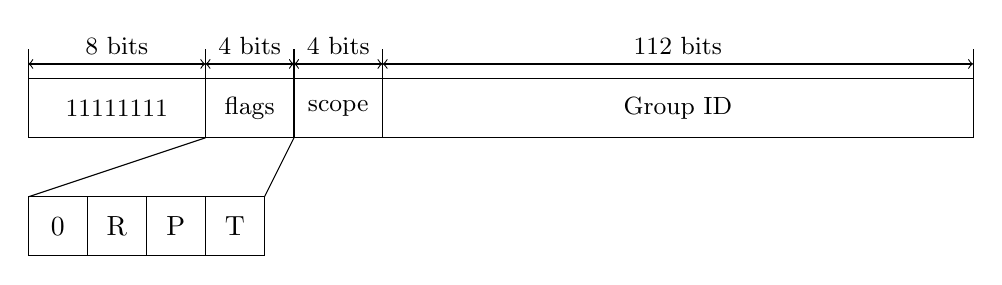
\begin{tikzpicture}[scale=0.75]
		\draw (0,2) rectangle (16,3);
		\draw (0,3) -- ++(0,0.5);
		\draw (3,2) -- ++(0,1.5);
		\draw (4.5,2) -- ++(0,1.5);
		\draw (6,2) -- ++(0,1.5);
		\draw (16,3) -- ++(0,0.5);
		\node at (1.5, 2.5) {\small 11111111};
		\node at (3.75, 2.5) {\small flags};
		\node at (5.25, 2.5) {\small scope};
		\node at (11, 2.5) {\small Group ID};
		\draw[<->] (0,3.25) -- ++(3,0) node[midway, above] {\small 8 bits};
		\draw[<->] (3,3.25) -- ++(1.5,0) node[midway, above] {\small 4 bits};
		\draw[<->] (4.5,3.25) -- ++(1.5,0) node[midway, above] {\small 4 bits};
		\draw[<->] (6,3.25) -- (16,3.25) node[midway, above] {\small 112 bits};

		\draw (3,2) -- (0,1);
		\draw (4.5,2) -- (4,1);
		\draw (0,0) rectangle (4,1);
		\node at (0.5,0.50) {0};
		\draw (1,0) -- ++(0,1);
		\node at (1.5,0.50) {R};
		\draw (2,0) -- ++(0,1);
		\node at (2.5,0.50) {P};
		\draw (3,0) -- ++(0,1);
		\node at (3.5,0.50) {T};
	\end{tikzpicture}
	\end{center}
	\caption{Multicast address}
	\label{fig:ipv6_multicast_addr}
\end{figure}